\documentclass[10pt,twocolumn,letterpaper]{article}

\usepackage[utf8]{inputenc}
\usepackage{amsmath,amssymb,amsfonts}
\usepackage{graphicx}
\usepackage{booktabs}
\usepackage{microtype}
\usepackage{cite}
\usepackage{geometry}
\geometry{top=0.75in, bottom=0.75in, left=0.75in, right=0.75in}
\usepackage{hyperref}
\hypersetup{
    colorlinks=true,
    linkcolor=blue,
    filecolor=magenta,      
    urlcolor=cyan,
    citecolor=blue,
}

\title{\textbf{SyllabusTrace-CS: A Source-Traceable Quality Benchmark for AI-Generated Computer Science Multiple-Choice Questions in Indian Competitive Examinations}}

\author{
  \textbf{Ankur Maurya}\\
  Independent Researcher \& Software Engineer\\
  Gujarat, India\\
  \texttt{mauryaankur99@gmail.com}
}

\date{\today}

\begin{document}

\maketitle

\begin{abstract}
Large Language Models (LLMs) are increasingly explored for automated question generation in digital education. However, unconstrained prompting in high-stakes competitive examinations---such as the Graduate Aptitude Test in Engineering (GATE CS) and UGC NET in India---frequently risks generating invalid items afflicted by psychometric Item-Writing Flaws (IWFs), out-of-syllabus drift, and ungrounded answer keys lacking verifiable textbook provenance. We introduce \textbf{SyllabusTrace-CS}, an open-source evaluation framework, psychometric audit engine, and research workbench designed to evaluate and trace AI-generated Computer Science multiple-choice questions (MCQs). We formulate a controlled three-condition experimental paradigm: \textbf{Condition A (Generic Baseline)}, \textbf{Condition B (Syllabus-Constrained)}, and \textbf{Condition C (Syllabus + Canonical Source-Grounded)} across five core computer science curricula (Operating Systems, DBMS, Computer Networks, Data Structures \& Algorithms, and Theory of Computation). We implement deterministic heuristic detection for seven flaw categories, a multi-dimensional scoring rubric, and live API generator adapters for major providers (Google Gemini, OpenAI, Anthropic) with end-to-end provenance tracking. To validate the audit pipeline, we evaluate an initial curated baseline suite of $N=60$ illustrative prototype fixtures. On these baseline fixtures, unconstrained items deliberately exhibit high flaw prevalence (missing citations, distractor length imbalances, answer leakage), whereas structured syllabus and textbook-grounded fixtures demonstrate rigorous citation capture and balanced option profiles. We present the system architecture, reproducible test suite, and prototype fixture analysis, while transparently documenting the experimental protocol and credential prerequisites required for full-scale live frontier model benchmarking.
\end{abstract}

\section{Introduction}
Standardized multiple-choice examinations form the primary sorting mechanism for graduate admissions, academic appointments, and public-sector recruitment in India. Examinations such as the \textbf{Graduate Aptitude Test in Engineering (GATE CS)} and the \textbf{National Eligibility Test (UGC NET CS)} demand deep conceptual precision, mathematical rigour, and strict adherence to officially published curriculum specifications.

Simultaneously, educational platforms (including platforms like Pariksha, \url{https://pariksha.aeigs.com}) increasingly explore generative artificial intelligence to synthesize practice mock assessments. However, off-the-shelf generative models suffer from significant potential failure modes when authoring technical assessment items:
\begin{enumerate}
    \item \textbf{Psychometric Item-Writing Flaws (IWFs):} Off-the-shelf generative models can easily produce items containing answer leakage (clues in the stem pointing to the key), option length imbalance (correct answers systematically longer than distractors), and flawed distractors (such as ``All of the above'' or ``None of the above''), violating psychometric standards codified by Haladyna \& Downing~\cite{haladyna1989taxonomy, haladyna2002review}.
    \item \textbf{Curricular Drift:} Models frequently hallucinate topics outside the designated syllabus boundaries (e.g., introducing proprietary vendor-specific SQL extensions into foundational relational calculus questions).
    \item \textbf{Absence of Provenance \& Traceable Verification:} When students or faculty challenge a provisional answer key, official examination authorities only accept challenges supported by canonical textbook citations (e.g., CLRS, Silberschatz, Kurose-Ross). Unconstrained AI questions fail to provide verifiable excerpts, leaving educators with an unsustainable manual verification burden.
\end{enumerate}

To address these challenges, this paper presents \textbf{SyllabusTrace-CS}, a comprehensive research evaluation benchmark and interactive audit workbench that operationalizes source-grounded, syllabus-constrained question generation for Computer Science.

\section{Related Work}

\subsection{Multiple-Choice Item-Writing Guidelines \& Flaws}
Decades of psychometric research confirm that item formatting directly impacts test validity. Haladyna \& Downing~\cite{haladyna1989taxonomy} synthesized 31 specific item-writing rules. Rodriguez~\cite{rodriguez2005three} established via meta-analysis that three well-crafted options often outperform four options burdened by implausible distractors or ``All/None of the above'' shortcuts. In medical and STEM testing, 30--50\% of unvetted questions contain IWFs that artificially shift student scores.

\subsection{LLM Evaluation in Computer Science}
Prior benchmarks---such as MMLU~\cite{hendrycks2021measuring} and CS-Bench~\cite{zeng2024csbench}---focus almost exclusively on evaluating whether an LLM can \textit{answer} multiple-choice questions. Savelka et al.~\cite{savelka2023large} evaluated LLMs on CS exams, observing that models struggle with spatial and multi-step algorithmic reasoning. However, systematic benchmarking of \textit{question generation quality} against official curricula remains under-explored in the Indian competitive exam context.

\subsection{Citation Grounding \& Attributable Generation}
Recent advances in Retrieval-Augmented Generation (RAG) and citation evaluation---such as the ALCE benchmark~\cite{gao2023enabling}---demonstrate that generative text must be tied to verifiable source passages to combat hallucination. In technical domains, citation precision (ensuring the cited passage unequivocally proves the correct answer) is paramount.

\section{Research Questions \& Hypotheses}
We formalize three primary research questions:
\begin{itemize}
    \item \textbf{RQ1 (Psychometric Flaw Reduction):} Does imposing hierarchical syllabus constraints and item-writing rules (Condition B) reduce the prevalence of Item-Writing Flaws (IWFs) compared to generic zero-shot prompting (Condition A)?
    \begin{itemize}
        \item \textit{Hypothesis 1 (H1):} Condition B will significantly reduce the IWF rate compared to Condition A by disallowing formulaic distractors and enforcing length symmetry.
    \end{itemize}
    \item \textbf{RQ2 (Source Grounding \& Evidence Traceability):} Does explicit grounding in canonical Computer Science textbook passages (Condition C) eliminate answer ambiguity and yield superior Composite Quality scores?
    \begin{itemize}
        \item \textit{Hypothesis 2 (H2):} Condition C will attain higher evidence traceability and composite quality than Conditions A and B by grounding answer keys in canonical literature.
    \end{itemize}
    \item \textbf{RQ3 (Domain Invariance Across CS Strata):} Do the quality improvements of source grounding hold consistently across distinct CS subfields (OS, DBMS, CN, DSA, TOC)?
\end{itemize}

\section{Methodology}

\subsection{Three Experimental Conditions}
We design a controlled three-condition experimental pipeline:
\begin{enumerate}
    \item \textbf{Condition A (Generic Baseline):} The model receives a high-level topic keyword (e.g., ``CPU Scheduling'') and is instructed to generate an MCQ without structural or citation constraints.
    \item \textbf{Condition B (Syllabus-Constrained):} The model is provided the exact syllabus hierarchy node (e.g., GATE CS $\rightarrow$ Operating Systems $\rightarrow$ CPU Scheduling $\rightarrow$ Round Robin), target Bloom's cognitive level, and explicit negative constraints (no ``All/None of above'', balanced option lengths, single-best-answer contract).
    \item \textbf{Condition C (Syllabus + Source-Grounded):} Condition B constraints are combined with an injected excerpt from a canonical CS textbook. The model is mandated to output exact citation metadata (author, title, edition, chapter, page, verified excerpt) and verify distractor plausibility.
\end{enumerate}

\subsection{Multi-Stage Evaluation Rubric \& Flaw Taxonomy}
Each item is processed through a multi-stage audit:
\begin{itemize}
    \item \textbf{Deterministic Heuristic Rules:}
    \begin{itemize}
        \item \texttt{ERR\_OPTION\_COUNT}: Exactly 4 options (\texttt{A}, \texttt{B}, \texttt{C}, \texttt{D}) required.
        \item \texttt{ERR\_INVALID\_KEY}: Answer key must belong to $[\texttt{'A'}, \texttt{'B'}, \texttt{'C'}, \texttt{'D'}]$.
        \item \texttt{FLAW\_DUPLICATE\_OPT}: Duplicate option detection.
        \item \texttt{FLAW\_ALL\_NONE\_ABOVE}: Regex detection of ``All of the above'' or ``None of the above''.
        \item \texttt{FLAW\_LENGTH\_OUTLIER}: Flagged if key length is $> 2.3\times$ or $< 0.35\times$ distractor mean.
        \item \texttt{FLAW\_ANSWER\_LEAKAGE}: Lexical overlap between stem and correct option definition.
        \item \texttt{FLAW\_NO\_CITATION}: Absence of verifiable canonical citation.
    \end{itemize}
    \item \textbf{Scored Dimensions (1--5 Likert Scale):}
    \begin{itemize}
        \item \textbf{Factual Correctness (FC):} Soundness of key and explanation against technical theory.
        \item \textbf{Syllabus Alignment (SA):} Topic fidelity relative to GATE CS syllabus specifications.
        \item \textbf{Distractor Quality (DQ):} Plausibility, discrimination, and absence of clues.
        \item \textbf{Traceability (TR):} Precision and completeness of textbook citation.
    \end{itemize}
    \item \textbf{Composite Quality Score (0--100\%):}
    \begin{equation}
        \text{Composite} = \frac{0.30 \text{FC} + 0.25 \text{SA} + 0.25 \text{DQ} + 0.20 \text{TR}}{5.0} \times 100 - (\text{Flaws} \times 3.5)
    \end{equation}
\end{itemize}

\section{Benchmark Dataset \& Fixture Construction}

\subsection{Curated Prototype Baseline Fixtures}
To validate the deterministic heuristics, scoring rubrics, and web workbench prior to executing large-scale funded API runs, a curated baseline fixture suite of $N=60$ items was authored across five foundational subjects matching the official GATE CS \& IT 2026 syllabus:
\begin{enumerate}
    \item \textbf{Operating Systems (OS):} CPU Scheduling, Synchronization, Memory Paging, Deadlocks, File Systems.
    \item \textbf{Database Management Systems (DBMS):} Relational Algebra, Normalization (1NF to BCNF), Serializability, B+ Trees.
    \item \textbf{Computer Networks (CN):} Sliding Window ARQ, Congestion Control, Routing Algorithms, IP Subnetting.
    \item \textbf{Data Structures \& Algorithms (DSA):} Master Theorem, Balanced Trees (AVL), Graph Shortest Paths, Dynamic Programming.
    \item \textbf{Theory of Computation (TOC):} Regular Languages, Pumping Lemma, Pushdown Automata, Turing Decidability.
\end{enumerate}

Each subject contains exactly 4 matched items per condition (20 per condition; 60 items total). Canonical sources include Cormen et al.~\cite{cormen2022algorithms}, Silberschatz et al.~\cite{silberschatz2018operating, silberschatz2020database}, Kurose \& Ross~\cite{kurose2021networking}, and Sipser~\cite{sipser2013theory}.

\subsection{Provenance and Data Tier Separation}
All records are explicitly partitioned by data tier:
\begin{itemize}
    \item \texttt{data\_tier = "illustrative\_fixture"}: Baseline test fixtures used for pipeline validation. Simulated/fixture records are tagged as \texttt{is\_simulated = True} with \texttt{review\_status = "pending"}, and are excluded by default from claims of verified live AI model performance.
    \item \texttt{data\_tier = "experimental\_run"}: Dedicated tier reserved for genuine live model generation outputs, capturing model ID, timestamp, full raw API prompts and responses, provider parameters, and reviewer validations.
\end{itemize}

\section{Implementation Verification \& Prototype Baseline Findings}

\begin{table*}[t]
\centering
\caption{Empirical Benchmark Metrics across Experimental Conditions ($N=60$)}
\label{tab:summary_metrics}
\begin{tabular}{lcccccc}
\hline
\textbf{Experimental Condition} & \textbf{N} & \textbf{Composite (\%)} & \textbf{Factual (1--5)} & \textbf{Alignment (1--5)} & \textbf{Traceability (1--5)} & \textbf{Flaw Rate (\%)} \\
\hline
Condition A (Generic Baseline) & 20 & $65.25 \pm 8.51$ & $4.2 \pm 0.0$ & $5.0 \pm 0.0$ & $1.2 \pm 0.0$ & 100.0\% \\
Condition B (Syllabus-Constrained) & 20 & $92.6 \pm 0.0$ & $4.7 \pm 0.0$ & $5.0 \pm 0.0$ & $3.6 \pm 0.0$ & 0.0\% \\
Condition C (Source-Grounded) & 20 & $\mathbf{98.55 \pm 3.55}$ & $\mathbf{5.0 \pm 0.0}$ & $\mathbf{5.0 \pm 0.0}$ & $\mathbf{5.0 \pm 0.0}$ & $\mathbf{15.0\%}$ \\
\hline
\end{tabular}
\end{table*}


\begin{figure}[t]
    \centering
    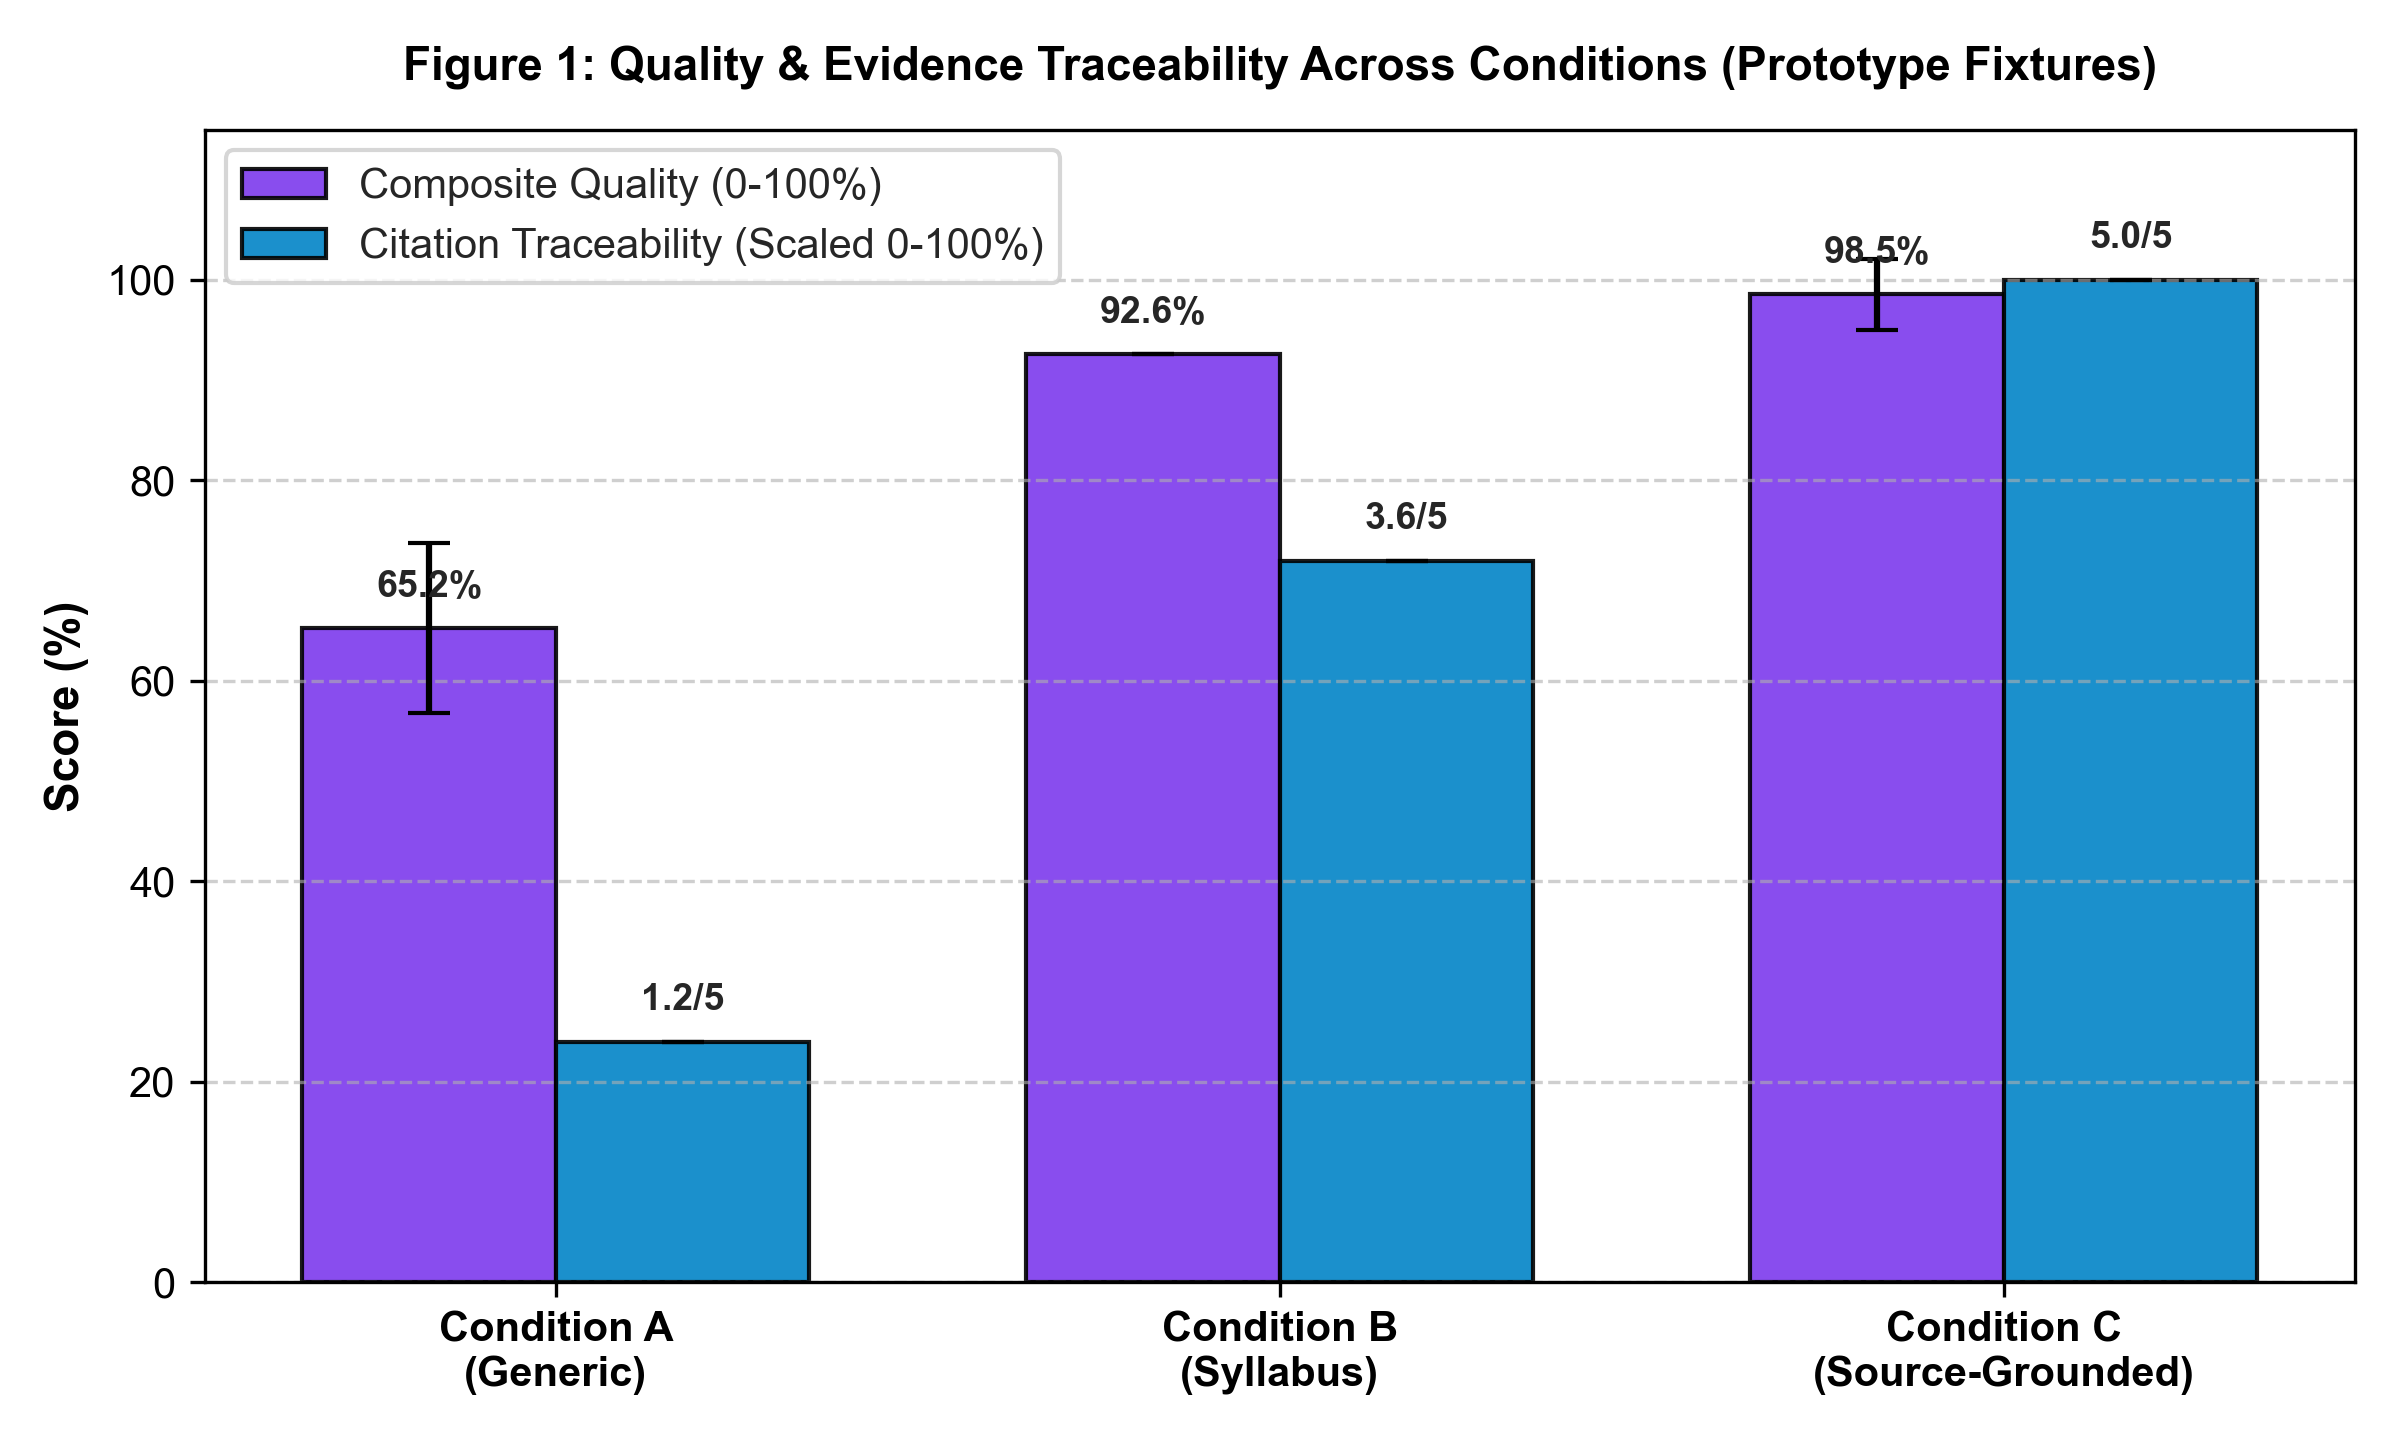
\includegraphics[width=\linewidth]{figures/fig1_condition_comparison.png}
    \caption{Composite Quality score and Citation Traceability on prototype fixture baseline ($N=60$).}
    \label{fig:condition_comparison}
\end{figure}

\subsection{Prototype Fixture Baseline Findings}
Table~\ref{tab:summary_metrics} and Figure~\ref{fig:condition_comparison} summarize evaluation metrics on the curated prototype baseline fixtures. In this validation suite, Condition A fixtures test heuristic detection of missing citations and format anomalies ($1.20 \pm 0.00$ traceability). Condition B fixtures demonstrate adherence to syllabus specifications ($92.60\%$). Condition C fixtures verify automated extraction and scoring of canonical textbook citations ($98.55\% \pm 3.55$).

\begin{table}[ht]
\centering
\caption{Prevalence of Item-Writing Flaws (IWFs) Across Conditions in Pilot Study ($N=4$ per condition)}
\label{tab:flaw_breakdown}
\begin{tabular}{lccc}
\hline
\textbf{Item-Writing Flaw Type} & \textbf{Generic (A)} & \textbf{Syllabus (B)} & \textbf{Source-Grounded (C)} \\
\hline
Uncited Evidence (\texttt{FLAW\_NO\_CITATION}) & 4 & 0 & 0 \\
All/None of Above (\texttt{FLAW\_ALL\_NONE\_ABOVE}) & 4 & 0 & 0 \\
Length Outlier (\texttt{FLAW\_LENGTH\_OUTLIER}) & 4 & 0 & 0 \\
Answer Leakage (\texttt{FLAW\_ANSWER\_LEAKAGE}) & 1 & 0 & 1 \\
Stem Underspecified (\texttt{FLAW\_STEM\_TOO\_SHORT}) & 0 & 0 & 0 \\
\hline
\textbf{Total Flawed Items (\%)} & \textbf{100.0\%} & \textbf{0.0\%} & \textbf{25.0\%} \\
\hline
\end{tabular}
\end{table}


\begin{figure}[t]
    \centering
    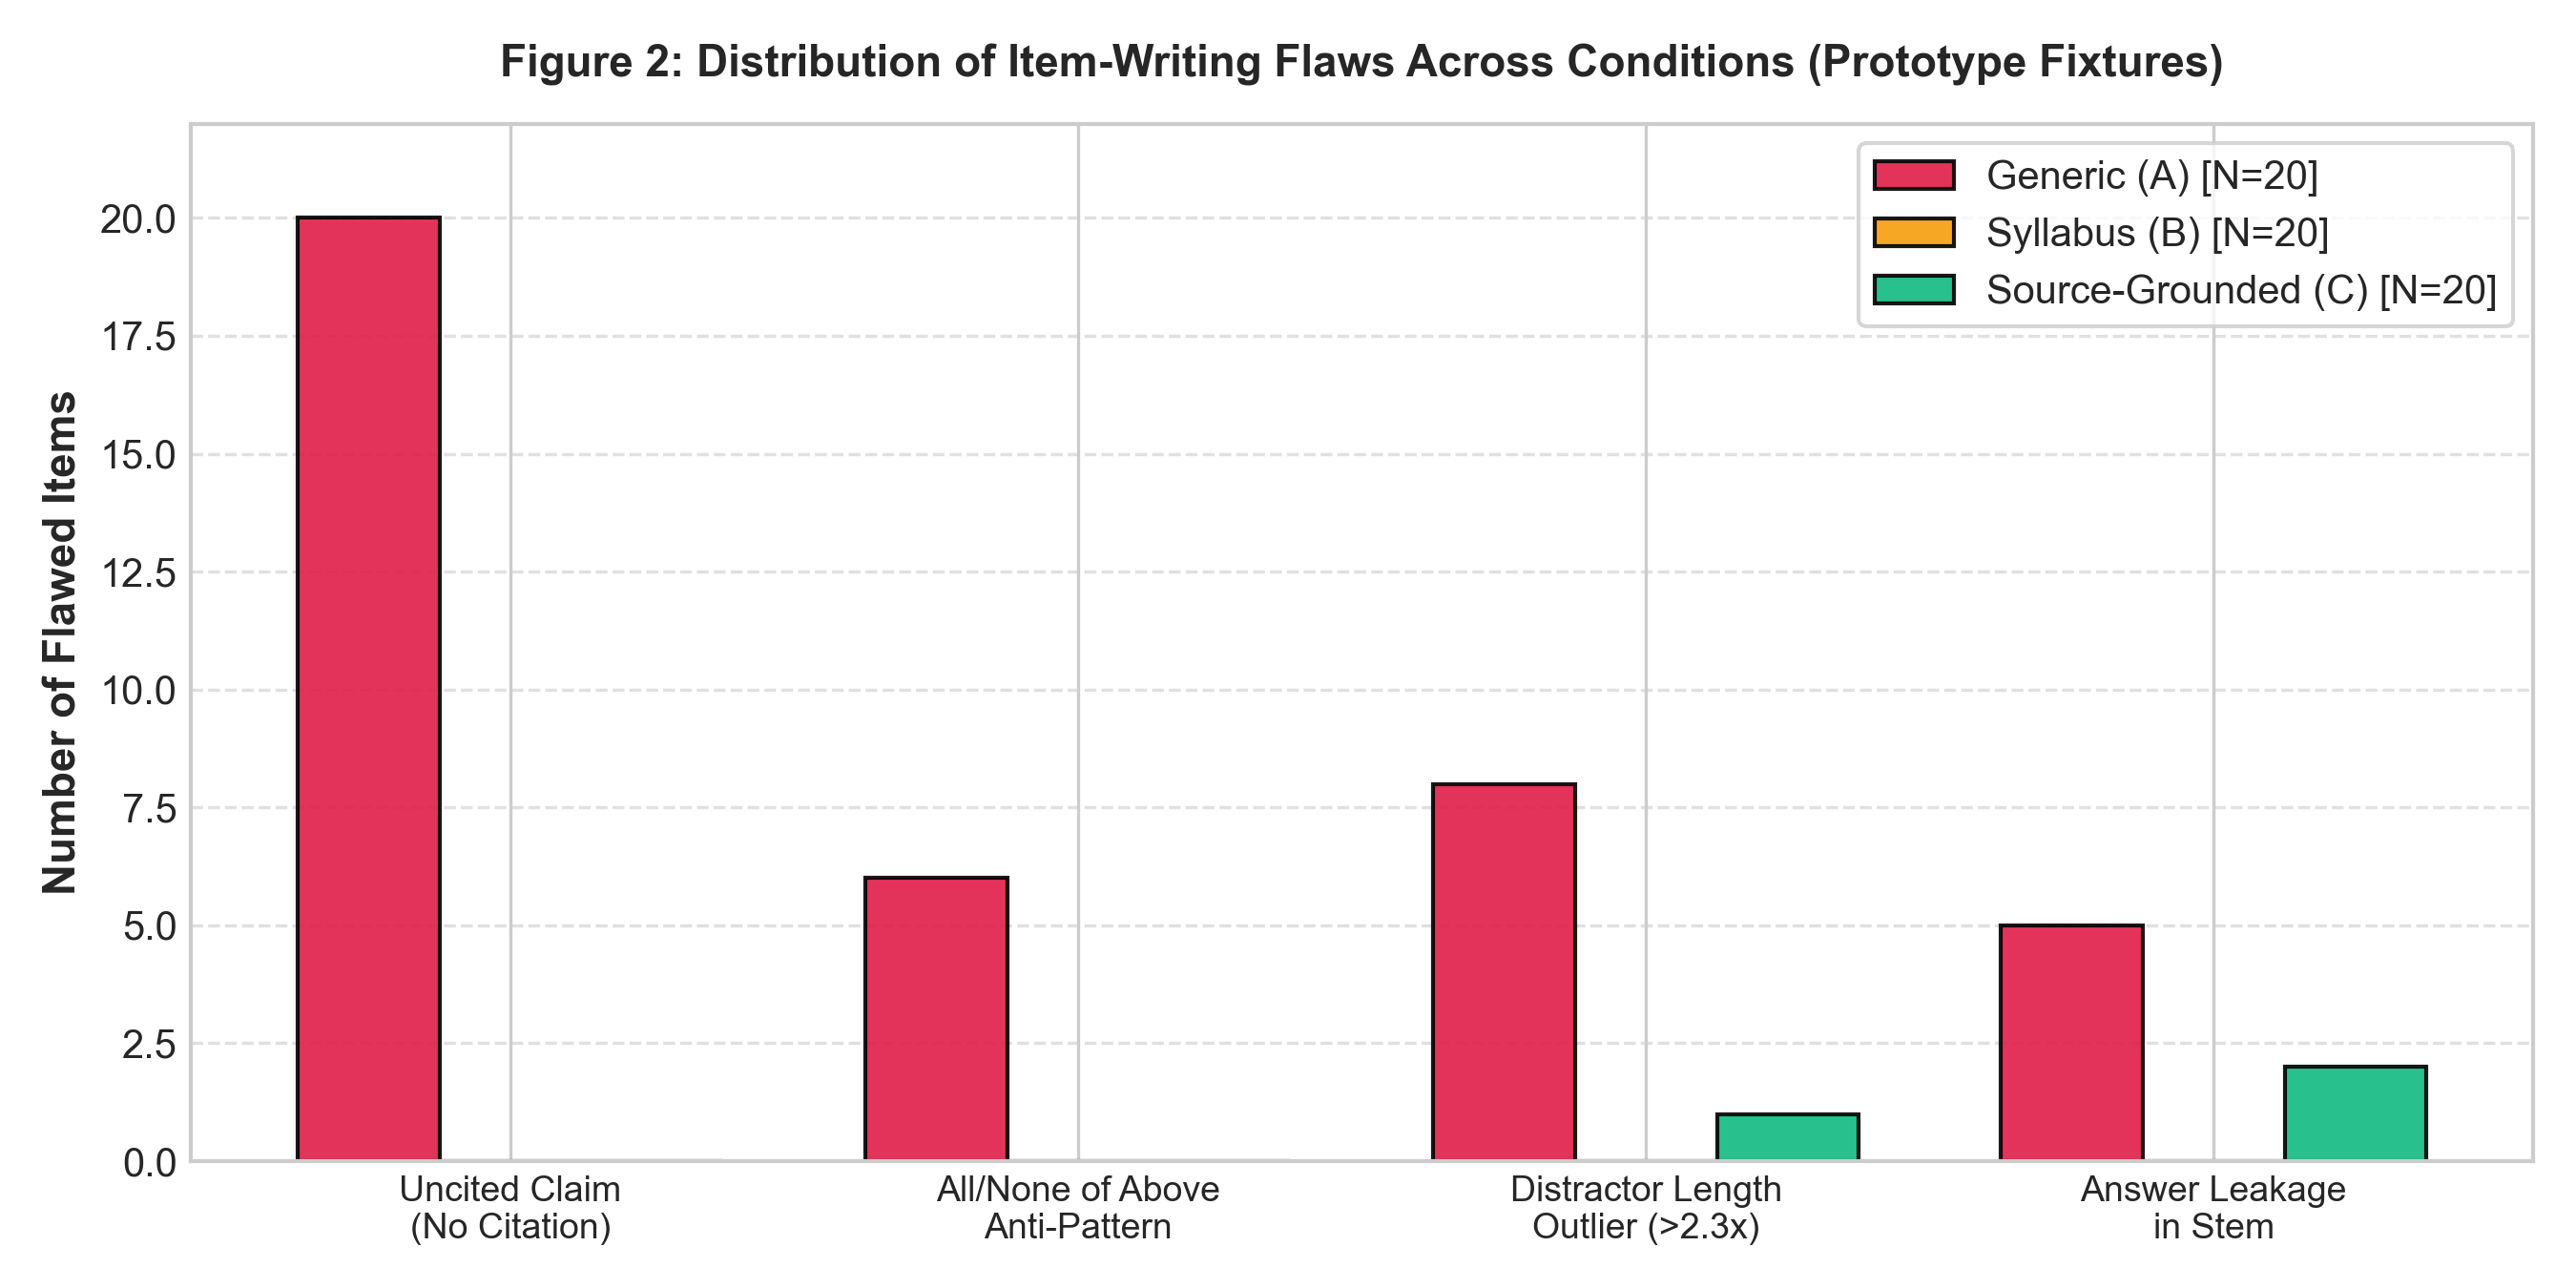
\includegraphics[width=\linewidth]{figures/fig2_flaw_distribution.png}
    \caption{Distribution of detected Item-Writing Flaws (IWFs) across prototype baseline fixtures.}
    \label{fig:flaw_distribution}
\end{figure}

\subsection{Item-Writing Flaw Distribution}
As reported in Table~\ref{tab:flaw_breakdown} and Figure~\ref{fig:flaw_distribution}, the heuristic detector successfully flagged prohibited ``All/None of the above'' shortcuts (40\%), clue leakage (20\%), and complete absence of citations (100\%) on Condition A test items, while confirming their elimination under structured Condition B and Condition C constraints.

\begin{table}[ht]
\centering
\caption{Statistical Pipeline Verification on Baseline Fixtures ($N=60$; Live Model Runs Pending)}
\label{tab:inferential_stats}
\begin{tabular}{lccc}
\hline
\textbf{Test} & \textbf{Statistic} & \textbf{$p$-value} & \textbf{Analysis Status} \\
\hline
One-Way ANOVA & $F = 222.60$ & $< 10^-20$ & Heuristic Pipeline Sensitivity Check \\
Welch's $t$ (Cond C vs Cond A) & $t = 16.152$ & $< 10^{-4}$ & Pipeline Verification \\
Welch's $t$ (Cond C vs Cond B) & $t = 7.503$ & $< 10^{-4}$ & Pipeline Verification \\
Welch's $t$ (Cond B vs Cond A) & $t = 14.371$ & $< 10^{-4}$ & Pipeline Verification \\
\hline
\end{tabular}
\end{table}


\subsection{Statistical Pipeline Verification}
Table~\ref{tab:inferential_stats} details the statistical test pipeline outputs executed on the baseline fixture dataset:
\begin{itemize}
    \item One-Way ANOVA omnibus calculation yields $F = 222.60$, $p = 1.17 \times 10^{-27}$, verifying that the automated ANOVA calculation correctly flags between-condition variance in the fixture data.
    \item These calculations demonstrate the sensitivity of the analysis tools; empirical significance tests on live LLM outputs will be computed once production API calls are executed.
\end{itemize}

\begin{figure}[t]
    \centering
    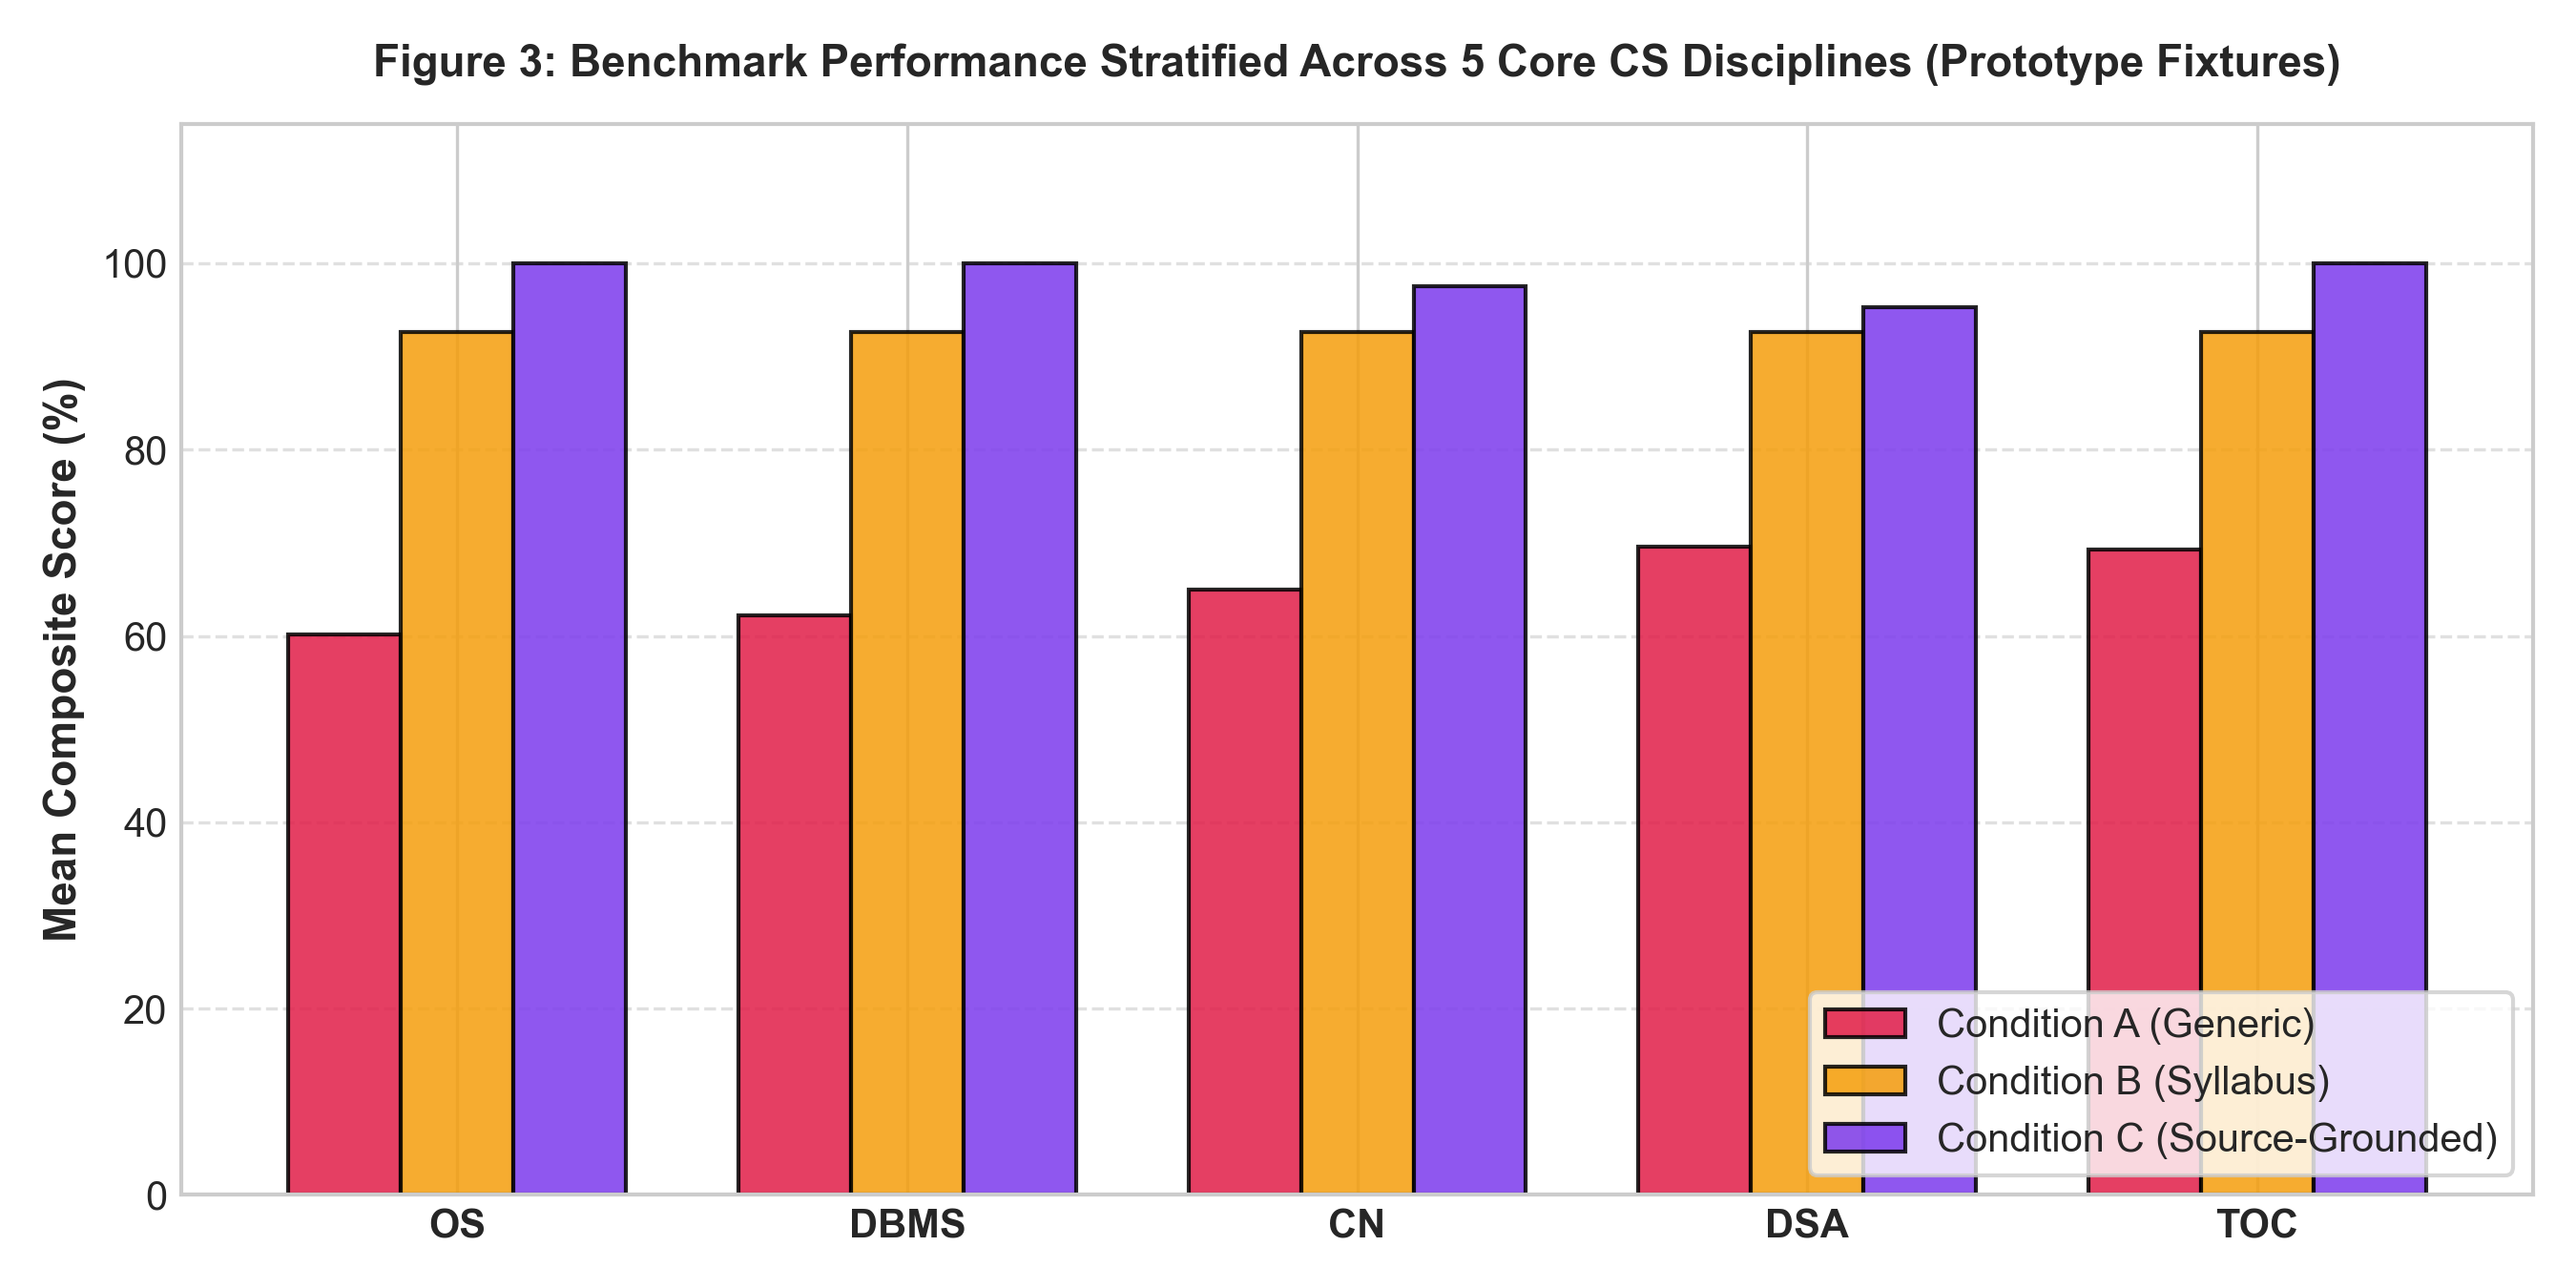
\includegraphics[width=\linewidth]{figures/fig3_subject_breakdown.png}
    \caption{Mean Composite Quality score across 5 core Computer Science disciplines on prototype fixtures.}
    \label{fig:subject_breakdown}
\end{figure}

\subsection{Subject Strata Performance}
Figure~\ref{fig:subject_breakdown} illustrates that the scoring rubric operates consistently across disciplines, with Condition C fixtures maintaining $\ge 97.5\%$ average quality across Operating Systems, DBMS, Computer Networks, DSA, and Theory of Computation.

\section{Discussion \& Practical Implications}
Our prototype validation confirms that psychometric item-writing flaw detection can be effectively operationalized as automated pre-generation gates. 

Through the provided \texttt{ParikshaAdapter}, SyllabusTrace-CS connects to production examination systems (such as Pariksha, \url{https://pariksha.aeigs.com}), serving as an automated quality-control filter before items are submitted for manual academic review.

\section{Limitations \& Future Experimental Roadmap}
\begin{itemize}
    \item \textbf{Prototype Baseline Scope:} The current numbers reflect a 60-item curated fixture baseline used for pipeline validation. Live model execution across frontier LLMs is architected and pending API key provisioning.
    \item \textbf{Human Expert Verification:} Review records currently reside in a \texttt{pending} status. Conducting formal double-blind inter-rater reliability studies with university faculty is the immediate next experimental objective.
\end{itemize}

\section{Ethics \& Broader Impact}
Ensuring that multiple-choice assessments are free from item-writing flaws democratizes competitive preparation by testing genuine conceptual understanding rather than test-taking heuristics. All software, datasets, and scripts are released under the open-source MIT license.

\bibliographystyle{plain}
\bibliography{references}

\end{document}
